%%%%%%%%%%%%%%%%%%%%%%%%%%%%%%%%%%%%%%%%%%%%%%%%%%%%%%%%%%%%%%%%%%%%%%%%%%%%%%%%%%%%
%Do not alter this block of commands.  If you're proficient at LaTeX, you may include additional packages, create macros, etc. immediately below this block of commands, but make sure to NOT alter the header, margin, and comment settings here. 
\documentclass[12pt]{article}
 \usepackage[margin=1in]{geometry} 
\usepackage{amsmath,amsthm,amssymb,amsfonts, enumitem, fancyhdr, color, hyperref,comment, graphicx, environ,mathtools, bbm, tikz, setspace, cleveref,listings, dcolumn}
\usepackage{array, multirow, caption, booktabs}
\usepackage{lscape}
\usepackage{ mathrsfs }
\usetikzlibrary{matrix,positioning}
\tikzset{bullet/.style={circle,draw=black,inner sep=8pt}}
\DeclareMathOperator*{\argmax}{arg\,max}
\DeclareMathOperator*{\argmin}{arg\,min}
\DeclareMathOperator*{\Var}{\text{Var}}
\DeclareMathOperator*{\Cov}{\text{Cov}}

\DeclarePairedDelimiter\norm{\lVert}{\rVert}%
\newtheorem{theorem}{Theorem}
\newtheorem{lemma}[theorem]{Lemma}
\DeclareMathOperator{\eps}{\varepsilon}
\doublespacing
\DeclarePairedDelimiter\abs{\lvert}{\rvert}%
\pagestyle{fancy}
\setlength{\headheight}{65pt}
\newenvironment{problem}[2][Problem]{\begin{trivlist}
\item[\hskip \labelsep {\bfseries #1}\hskip \labelsep {\bfseries #2.}]}{\end{trivlist}}
\newenvironment{sol}
    {\emph{Solution:}
    }
    {
    \qed
    }


%%%%%%%%%%%%%%%%%%%%%%%%%%%%%%%%%%%%%%%%%%%%%%%%%%%%%%%%%%%%%%%%%%%%%%%%%%%%%%%%%


\usepackage{xcolor}
 
 


%%%%%%%%%%%%%%%%%%%%%%%%%%%%%%%%%%%%%%%%%%%%%

\rhead{Asha Bharadwaj, Caitlin Dutta, John Higgins, Alexis Smith\\Econ 899 \\ 18 November, 2022} 

%%%%%%%%%%%%%%%%%%%%%%%%%%%%%%%%%%%%%%%%%%%%%


%%%%%%%%%%%%%%%%%%%%%%%%%%%%%%%%%%%%%%

\begin{document}
We consider a dynamic model of loan repayment. $T_i \in \{1,2,3,4\}$ denotes the observed loan duration, and $Y_{it}$ denotes an indicator variable equal to one if the loan is pre-paid at the end of period $t$. $T_i$ is related to $Y_{it}$ in the following manner:
\[T_i = \begin{cases} 1 \quad&\text{if } Y_{i0} = 0\\
    2 \quad&\text{if } Y_{i0} = 0 \text{ and } Y_{i1} = 1\\
    3 \quad&\text{if } Y_{i0} = Y_{i1}= 0 \text{ and } Y_{i2} = 1\\
    4 \quad&\text{if } Y_{i0} = Y_{i1} = Y_{i2} = 0
\end{cases}\]
We assume that, at each period $t$, a loan is repaid only if
\[\alpha_t + X_i \beta + Z_{it} \gamma + \eps_{it} < 0\]
Rearranging this, we find that the loan will be repaid only If
\[\eps_{it} < -\alpha_t - X_{i}\beta - Z_{it}\gamma\]
This means that a loan will \textit{not} be repaid in period $t$ if $\eps_{it} \geq -\alpha_t - X_{i}\beta - Z_{it}\gamma$.

We assume that $X_{i}$ is a time-invariant vector of borrow characteristics, $Z_{it}$ is a vector of time varying characteristics (such as the borrower's FICO score), and $\eps_{it} = \rho \eps_{i t-1} + \eta_{it}$ if $t > 1$ and $\eta_{it} \sim N(0,1)$. We assume that $\eps_{it} \sim N(0, \sigma^2_0)$, with $\sigma^2_0 = \frac{1}{(1-\rho)^2}$. 

Given this setup, we must derive the likelihood associated with loan duration $T_i$. I believe that the likelihood given in the problem set is not quite correct, so I have attempted to derive it based on the above assumptions.

We first wish to find the likelihood of observing $T_i = 1$ given $X_i, Z_i$, and $\theta$. $T_i = 1$ corresponds to the loan being paid off at $t = 0$. This means that 
\begin{align*} 
    P(T_i = 1 \mid X_i, Z_i, \theta) &= P(\alpha_0 + X_i \beta + Z_{i0} \gamma + \eps_{i0} < 0)\\
    &= P(\eps_{i0} < -\alpha_0 + -X_i \beta - Z_{i0} \gamma)\\
    &= \Phi\left(\frac{-\alpha_0 + -X_i \beta - Z_{i0} \gamma}{\sigma_0}\right)
\end{align*}
since $\eps_{i0} \sim N(0, \sigma^2_0)$ implies that $\frac{\eps_{i0}}{\sigma_0} \sim N(0,1)$. Hence, we have that
\[P(T_i = 1 X_i, Z_i, \theta) = \Phi\left(\frac{-\alpha_0 + -X_i \beta - Z_{i0} \gamma}{\sigma_0}\right)\]


We now must find $P(T_i = 2 \mid X_i, Z_i, \theta)$. $T_i = 2$ corresponds to the loan not being repaid in $t = 0$ and being repaid in $t = 1$. Thus, we have that
\begin{align*}
    P(T_i = 2 \mid X_i, Z_i, \theta) &= P(\alpha_0 + X_i \beta + Z_{i0} \gamma + \eps_{i0} \geq 0, \alpha_1 + X_i \beta + Z_{i1} \gamma + \eps_{i1} < 0)\\
    &= P( \eps_{i0} \geq -\alpha_0 - X_i \beta - Z_{i0} \gamma,  \eps_{i1} < -\alpha_1 - X_i \beta - Z_{i1} \gamma)\\
    &= P( \eps_{i0} \geq -\alpha_0 - X_i \beta - Z_{i0} \gamma,  \rho \eps_{i0} + \eta_{i1} < -\alpha_1 - X_i \beta - Z_{i1} \gamma)\\
    &= P( \eps_{i0} \geq -\alpha_0 - X_i \beta - Z_{i0} \gamma,   \eta_{i1} < -\alpha_1 - X_i \beta - Z_{i1}\gamma -\rho \eps_{i0} )\\
    &= \int_{-\alpha_0 - X_i\beta - Z_{i0}\gamma}^{\infty} \Phi(-\alpha_1 - X_i \beta - Z_{i1}\gamma - \rho \eps_{i0}) \frac{\phi(\eps_{i0}/\sigma_0)}{\sigma_0} \, d \eps_{i0}
\end{align*}
We now consider $P(T_i = 3 \mid X_i, Z_i, \theta)$. This corresponds to the loan not being repaid in $t = 0$ or $t=1$ and being repaid in $t = 2$. For compactness, we define $b_0 = - \alpha_0 - X_i \beta - Z_{i0}\gamma$, $b_1 = - \alpha_1 - X_i \beta - Z_{i1}\gamma$, and $b_2 = - \alpha_2 - X_i \beta - Z_{i2}\gamma$. We deduce the following:
\begin{align*}
    P(T_i = 3 \mid X_i, Z_i, \theta) &= P(\alpha_0 + X_i \beta + Z_{i0} \gamma + \eps_{i0} \geq 0, \alpha_1 + X_i \beta + Z_{i1} \gamma + \eps_{i1} \geq 0, \\
    &\qquad \text{ \& } \alpha_2 + X_i \beta + Z_{i2} \gamma + \eps_{i2} < 0 )\\
    &= P( \eps_{i0} \geq b_0,  \eps_{i1} \geq b_1, \eps_{i2}< b_2)\\
    &= P( \eps_{i0} \geq b_0,  \eps_{i1} \geq b_1, \eta_{i2} < b_2 - \rho \eps_{i1})\\
    &= \int_{b_0}^{\infty} \int_{b_1}^{\infty} \Phi(b_2 - \rho \eps_{i1})\phi(\eps_{i1} - \rho \eps_{i0}) \frac{\phi(\eps_{i0}/\sigma_0)}{\sigma_0} \, d \eps_{i1} d \eps_{i0}
\end{align*}
Finally, we find $P(T_i = 4 \mid X_i, Z_i, \theta)$. This corresponds to the loan not being paid off in $t = 0, 1,$ or 2. The setup is very similar as the previous one, but with a flipped inequality for $\eps_{i2}$:
\begin{align*}
    P(T_i = 4 \mid X_i, Z_i, \theta) &= P(\alpha_0 + X_i \beta + Z_{i0} \gamma + \eps_{i0} \geq 0, \alpha_1 + X_i \beta + Z_{i1} \gamma + \eps_{i1} \geq 0, \\
    &\qquad \text{ \& } \alpha_2 + X_i \beta + Z_{i2} \gamma + \eps_{i2} \geq 0 )\\
    &= P( \eps_{i0} \geq b_0,  \eps_{i1} \geq b_1, \eps_{i2}\geq b_2)\\
    &= P( \eps_{i0} \geq b_0,  \eps_{i1} \geq b_1, \eta_{i2} \geq b_2 - \rho \eps_{i1})\\
    &= \int_{b_0}^{\infty} \int_{b_1}^{\infty} [1 - \Phi(b_2 - \rho \eps_{i1})]\phi(\eps_{i1} - \rho \eps_{i0}) \frac{\phi(\eps_{i0}/\sigma_0)}{\sigma_0} \, d \eps_{i1} d \eps_{i0}
\end{align*}
Combining these and using the above definitions of $b_0, b_1,$ and $b_2$, the likelihood is given by the following:
\begin{align*}
    P(T_i \mid X_i, Z_i, \theta) &= \begin{cases}
        \Phi(b_0/\sigma_0) \quad &\text{if } T_i = 1\\
        \int_{b_0}^{\infty} \Phi(b_1 - \rho \eps_{i0}) \frac{\phi(\eps_{i0}/\sigma_0)}{\sigma_0} \, d \eps_{i0} \quad &\text{if } T_i = 2\\
        \int_{b_0}^{\infty} \int_{b_1}^{\infty} \Phi(b_2 - \rho \eps_{i1})\phi(\eps_{i1} - \rho \eps_{i0}) \frac{\phi(\eps_{i0}/\sigma_0)}{\sigma_0} \, d \eps_{i1} d \eps_{i0} \quad &\text{if } T_i = 3\\
        \int_{b_0}^{\infty} \int_{b_1}^{\infty} [1 - \Phi(b_2 - \rho \eps_{i1})]\phi(\eps_{i1} - \rho \eps_{i0}) \frac{\phi(\eps_{i0}/\sigma_0)}{\sigma_0} \, d \eps_{i1} d \eps_{i0} \quad &\text{if } T_i = 4\\
    \end{cases}\\
    &\text{with } b_0 = - \alpha_0 - X_i \beta - Z_{i0}\gamma\\ 
    & \qquad b_1 = - \alpha_1 - X_i \beta - Z_{i1}\gamma\\
    & \qquad b_2 = - \alpha_2 - X_i \beta - Z_{i2}\gamma
\end{align*}

\begin{problem}{1}
\end{problem}
\begin{sol}
    We wrote a routine which evaluates the log-likelihood function using Gaussian quadrature. We used nodes and weights with precision of 20. We find that the log-likelihood of the initial parameter vector with $\alpha_0 = 0$, $\alpha_1 = -1$, $\alpha_2 = -1$, $\beta_0$, $\gamma = 0.3$, and $\rho = 0.5$ is equal to $-13598.877$. We plot the histogram of likelihoods for each outcome below:
    \begin{center}
        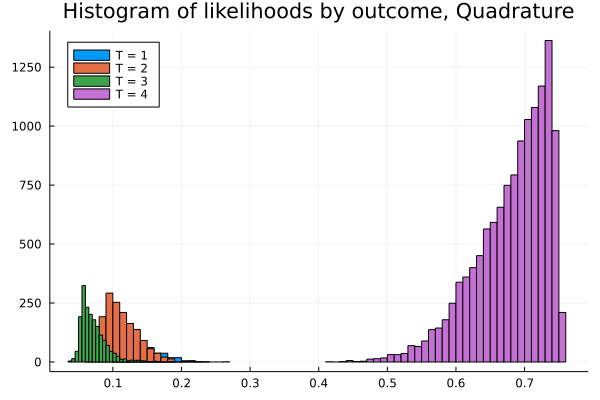
\includegraphics[scale=0.5]{Quadrature_ll.png}
    \end{center}
\end{sol}
\begin{problem}{2}
\end{problem}
\begin{sol}
    We now provide a routine which evaluates the log-likelihood using the GHK method. We create random samples from target distributions by first using Halton sequences to generate uniform draws from the interval $[0,1]$ and then transforming these draws using the quantile function of the specified distribution. 

    As previously, the likelihoods of each outcome can be written in the following form:
    \begin{align*}
        P(T_i \mid X_i, Z_i, \theta) &= \begin{cases}
            \Phi(b_0/\sigma_0) \quad &\text{if } T_i = 1\\
            P( \eps_{i0} \geq b_0,   \eps_{i1} < b_1) \quad &\text{if } T_i = 2\\
            P( \eps_{i0} \geq b_0,  \eps_{i1} \geq b_1, \eps_{i2} < b_2) \quad &\text{if } T_i = 3\\
            P( \eps_{i0} \geq b_0,  \eps_{i1} \geq b_1, \eps_{i2} \geq b_2) \quad &\text{if } T_i = 4
        \end{cases}\\
        &\text{with } b_0 = - \alpha_0 - X_i \beta - Z_{i0}\gamma\\ 
        & \qquad b_1 = - \alpha_1 - X_i \beta - Z_{i1}\gamma\\
        & \qquad b_2 = - \alpha_2 - X_i \beta - Z_{i2}\gamma
    \end{align*}
    We will rewrite each of these likelihoods as the product of independent (conditional) probabilities. The likelihood for $T_i = 2$ can be rewritten as the following:
    \begin{align*} 
        P(T_i = 2 \mid X_i, Z_i, \theta) &= P( \eps_{i0} \geq b_0,   \eps_{i1} < b_1 \gamma) \\
        &=  P(\eps_{i0} \geq b_0) P(\eps_{i1} < b_1 \mid \eps_{i0} \geq b_0)\\
        &= [1-\Phi(b_0/\sigma)] P(\eta_{i1} < b_1 - \rho \eps_{i0} \mid \eps_{i0} \geq b_0)\\
        &= [1-\Phi(b_0/\sigma)] \Phi(b_1 - \rho \eps_{i0} \mid \eps_{i0} \geq b_0)
    \end{align*}
    To compute the above likelihood, we must sample $\eps_{i0}$ from its (truncated) distribution and find the sample average of the likelihood evaluated at each sampled $\eps_{i0}$. Since we need $\eps_{i0} \geq b_0$, $\eps_{i0}$ will be drawn from a truncated normal distribution with mean 0, variance $\sigma_0^2$, and support $[b_0, \infty)$. Since $\eps_{i0} = \sigma \eta_{i0}$ where $\eta_{i0} \sim N(0,1)$, we can draw $\eps_{i0}$ from a truncated normal distribution with mean 0, variance 1, and support $[b_0/\sigma, \infty)$ and scale by $\sigma$ to get $\eps_{i0}$. 

    We draw $\eta_{i0}$ using the following procedure. For any $q \in [0,1]$ (ours will be randomly generated using Halton sequences), we let
    \[q = \frac{\Phi(\eta_{i0}) - \Phi(b_0/\sigma)}{1 - \Phi(b_0/\sigma)} \]
    Then, inverting this and solving for $\eta_{i0}$, we obtain
    \[\eta_{i0} = \Phi^{-1}[\Phi(b_0/\sigma) + q (1-\Phi(b_0/\sigma))]\]
    Finally, we scale by $\sigma$ to get $\eps_{i0} = \sigma \eta_{i0}$. This gives us a draw from the desired truncated distribution for $\eta_{i0}$. Let $\{q_k\}_{k=1}^{100}$ be drawn uniformly from $[0,1]$ and $ \{\eta_{i0}^k\}_{k=1}^{100}$ be the corresponding draws using the above procedure. The simulated likelihood of $P(T_i = 2 \mid X_i, Z_i, \theta)$ is the following:
    \[\hat{P}(T_i = 2 \mid X_i, Z_i, \theta) = \frac{1}{100} \sum_{i=1}^n [1-\Phi(b_0/\sigma)] \Phi(b_1 - \rho \eps_{i0}^k) \]
    
    We do a similar procedure for $T_i = 3$. Rewriting the likelihood as the product of conditional probabilities, we obtain:
    \begin{align*}
        P(T_i = 3  \mid X_i, Z_i, \theta)  &= P( \eps_{i0} \geq b_0,  \eps_{i1} \geq b_1, \eps_{i2} < b_2) \\
        &= [1-\Phi(b_0/\sigma)] P(\eta_{i1} \geq b_1 - \rho \eps_{i0} \mid \eps_{i0} \geq b_0) \\
        &\times P(\eta_{i2} < b_2 - \rho \eps_{i1} \mid \eps_{i1} \geq b_1- \rho \eps_{i0}, \eps_{i0} \geq b_0 )\\
        &= [1-\Phi(b_0/\sigma)] [1 - \Phi(b_1 - \rho \eps_{i0})] \Phi(b_2 - \rho \eps_{i1})
    \end{align*}
    where $\eps_{i0} \geq b_0$ and $\eps_{i1} \geq b_1$ in the last line.    
    
    Here, we must draw two samples recursively. First, we draw $\eps_{i0}$ as outlined in the previous section. Then, we must draw $\eps_{i1}$ such that $\eps_{i1} \geq b_1$. Note that since $\eps_{i1} = \rho \eps_{i0} + \eta_{i1}$, this is equivalent to drawing $\eta_{i1} \geq b_1 - \rho \eps_{i0}$. Thus, we first draw $\eta_{i1}$ from a truncated $N(0,1)$ distribution with support $[b_1 - \rho \eps_{i0}, \infty)$. Using our Halton sequence, we generate a random $q \in [0,1]$ and use this to find the corresponding $\eta_{i1}$:
    \[q = \frac{\Phi(\eta_{i1}) - \Phi(b_1 - \rho \eps_{i0})}{1 - \Phi(b_1 - \rho \eps_{i0})} \iff \eta_{i1} =  \Phi^{-1}[\Phi(b_1 - \rho \eps_{i0}) + q (1-\Phi(b_1 - \rho \eps_{i0}))]\]
    Then, we apply the following transformation to obtain $\eps_{i1}$:
    \[\eps_{i1} = \rho \eps_{i0} + \eta_{i1}\]
    
    To find the simulated likelihood, we proceed as before. We generate two uniform random samples $\{q_k^1, q_k^2\}_{k=1}^{100}$ using Halton sequences and find the corresponding draws $\{\eps_{i0}^k, \eps_{i1}^k\}_{k=1}^{100}$ using the procedure outlined above. Then, the simulated likelihood is given by
    \[\hat{P}(T_i = 3 \mid X_i, Z_i, \theta) = \frac{1}{100} \sum_{k=1}^{100} [1-\Phi(b_0/\sigma)] [1 - \Phi(b_1 - \rho \eps_{i0}^k)] \Phi(b_2 - \rho \eps_{i1}^k)\]

    The sampling procedure for $T_i = 4$ is identical, and the simulated likelihood is given by
    \[\hat{P}(T_i = 4 \mid X_i, Z_i, \theta) =[1-\Phi(b_0/\sigma)] [1 - \Phi(b_1 - \rho \eps_{i0}^k)] [1 -\Phi(b_2 - \rho \eps_{i1}^k)]\]

    Using this procedure, we find that the log-likelihood of the initial parameter guess is $-13584.549$, which is very close to the log-likelihood obtained in the first part. The histogram of likelihoods by outcome is included below. It matches very closely with that of quadrature:
    \begin{center}
        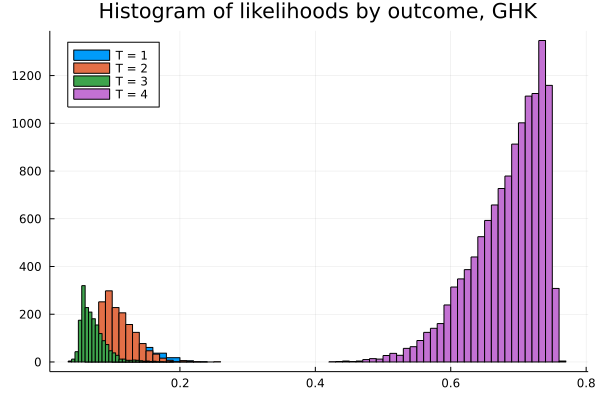
\includegraphics[scale=0.5]{GHK_ll.png}
    \end{center}
\end{sol}
\begin{problem}{3}
\end{problem}
\begin{sol}
    We provide a routine to evaluate the simulated log-likelihood using the Accept/Reject method with 100 simulation draws. We use Halton sequences with bases 7 and 11 for $\eps_{i0}$ and $\eps_{i1}$, respectively. We find that the simulated log-likelihood of the initial parameter vector is -13671.641, which is a bit different than the other two methods (but nonetheless relatively close in the grand scheme of things). We plot the histogram of likelihoods by outcome below:
    \begin{center}
        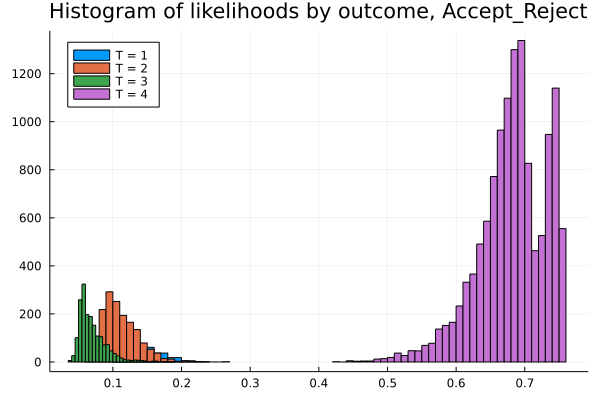
\includegraphics[scale=0.5]{Accept_Reject_ll.png}
    \end{center}
    We see that this histogram is a bit different from the previous two methods. This is reasonable, since the draws are random and thus number of draws which are accepted is also random. As such, the simulated likelihood may be taking an average over far fewer observations, leading to more noise in the estimate. We contrast this with GHK, which always has a sample size of 100 for each observation.
\end{sol}
\begin{problem}{4}
\end{problem}
\begin{sol}
    We compare the estimates from GHK and Accept/Reject with those obtained using quadrature. 

In the first figure, we plot the simulated likelihoods for quadrature on the horizontal axis and the simulated likelihoods for GHK on the vertical axis. The simulated likelihoods for GHK lie almost exactly on the 45-degree line, indicating that the simulated likelihoods are virtually identical to those found using quadrature. This is consistent with the fact that their histograms were virtually identical.
    \begin{center}
        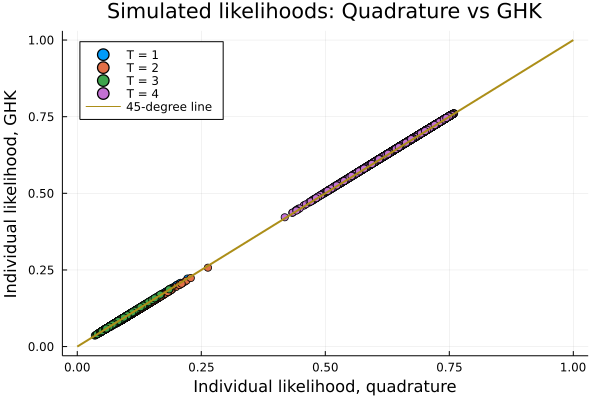
\includegraphics[scale=0.5]{GHK_comp.png}
    \end{center}
In the second figure, we plot the simulated likelihoods for quadrature on the horizontal axis and the simulated likelihoods for Accept/Reject on the vertical axis. We see that Accept/Reject is a bit less similar than GHK was. As previously discussed, this is attributable to the fact that the effective sample size for A/R is smaller since some draws are rejected. This leads to less precise estimates of the simulated likelihood than the other two methods.

We now compare the time it took for each method to complete. Running each once after initially compiling, we find that quadrature took 1.142 seconds, GHK took 0.750 seconds, and Accept/Reject took 0.482 seconds. Using the @belapsed command to run each routine many times and find the minimum runtime, we find that quadrature took a minimum of 0.787 seconds, GHK took a minimum of 0.5003 seconds, and Accept/Reject took a minimum of 0.326 seconds. While A/R is fastest, it is also less consistent than the other methods. It seems like GHK is faster than quadrature. However, this performance advantage will be diminished somewhat when a larger sample is taken (as we usually would). Generally, my impression is that quadrature offers better precision versus taking random samples, so this may be an instance where the tradeoff between speed and precision must be made. 
    \begin{center}
        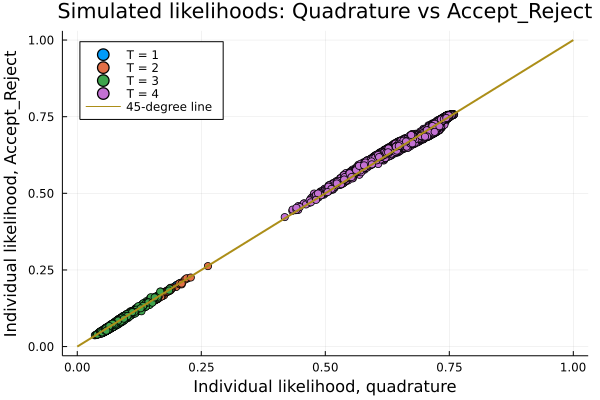
\includegraphics[scale=0.5]{Accept_Reject_comp.png}
    \end{center}
\end{sol}
\begin{problem}{5}
\end{problem}
\begin{sol}
We find that the simulated log-likelihood is maximized by the following parameter values:
\begin{table}[!htbp]
    \centering
    \begin{tabular}{|c|c|}
        \hline
        Parameter & Estimate\\
        \hline 
        $\alpha_0$ & 5.691 \\
$\alpha_1$ & 3.177 \\
$\alpha_2$ & 2.578 \\
score\_0 & 0.218 \\
rate\_spread & -0.325 \\
i\_large\_loan & -0.494 \\
i\_medium\_loan & -0.341 \\ 
i\_refinance & -0.082 \\
age_r & -0.208 \\
cltv & 0.065 \\
dti & -0.132 \\
cu & -0.523 \\
first\_mort\_r & -0.26 \\
i\_FHA & -0.371 \\
i\_open\_year\_2 &-0.62 \\
i\_open\_year\_3 &-0.162 \\
i\_open\_year\_4 &0.071 \\
i\_open\_year\_5 &0.081 \\
$\gamma$ & -0.098 \\
$\rho$ & 0.494 \\
\hline
    \end{tabular}
\end{table}
The maximimum log-likelihood evaluated at this parameter vector is -11374.07. It took approximately 36 minutes to get convergence using L-BFGS.

For fun, we plot the histogram of likelihoods at the optimal parameter vector below, as well as a comparison between the likelihoods at the optimal parameter vector vs the initial parameter vector:
\begin{center}
    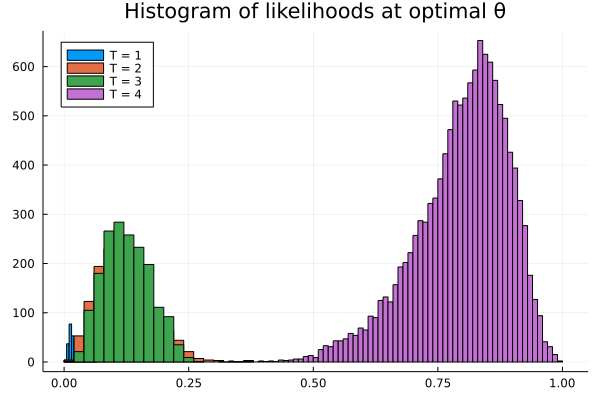
\includegraphics[scale=0.5]{opt_hist.png}
\end{center}
\begin{center}
    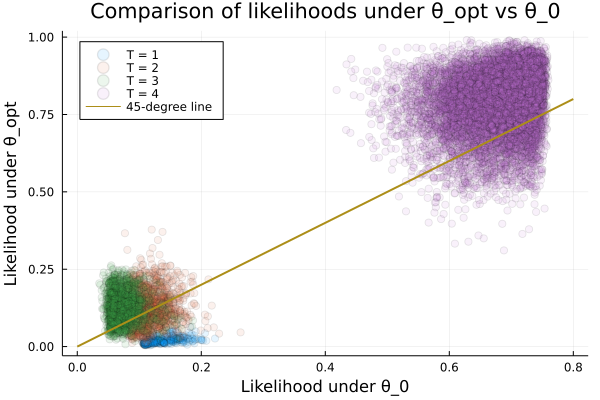
\includegraphics[scale=0.5]{scatter_comp.png}
\end{center}
We can see that the likelihoods tend to be higher under the optimal parameter vector (they'd better be!! I didn't spend 36 minutes running LBGFS for fun). This can be seen more clearly in the scatter plot, where the x coordinate of each dot is the likelihood of the observation under $\theta_0$ and the y coordinate is the likelihood of the observation under the optimal $\hat{\theta}$. the 45-degree line is also plotted (if a point lies above this line, then it has a higher likelihood under $\hat{\theta})$. We see that most of the points lie above the 45-degree line, except for T = 1 (which seems to be pretty low).
\end{sol}
\end{document}